\documentclass[onecolumn,10pt]{jhwhw}

\usepackage{epsfig} %% for loading postscript figures
\usepackage{amsmath}
\usepackage{graphicx}
\usepackage{grffile}
\usepackage{pdfpages}
\usepackage{algpseudocode}
\usepackage{wrapfig}
\usepackage{pgfplots}
\usepackage{amsfonts}
\usepackage{booktabs}
\usepackage{siunitx}
\usepackage{commath}
\usepackage{rotating}
\usepackage{url}
\usepackage{multimedia}
\usepackage{hyperref}
\usepackage{mathtools}

% Default fixed font does not support bold face
\DeclareFixedFont{\ttb}{T1}{txtt}{bx}{n}{12} % for bold
\DeclareFixedFont{\ttm}{T1}{txtt}{m}{n}{12}  % for normal

% Custom colors
\usepackage{color}
\usepackage{listings}
\usepackage{framed}
\usepackage{caption}
\usepackage{bm}
\captionsetup[lstlisting]{font={small,tt}}

\definecolor{mygreen}{rgb}{0,0.6,0}
\definecolor{mygray}{rgb}{0.5,0.5,0.5}
\definecolor{mymauve}{rgb}{0.58,0,0.82}

\lstset{ %
  backgroundcolor=\color{white},   % choose the background color; you must add \usepackage{color} or \usepackage{xcolor}
  basicstyle=\ttfamily\footnotesize, % the size of the fonts that are used for the code
  breakatwhitespace=false,         % sets if automatic breaks should only happen at whitespace
  breaklines=true,                 % sets automatic line breaking
  captionpos=b,                    % sets the caption-position to bottom
  commentstyle=\color{mygreen},    % comment style
  deletekeywords={...},            % if you want to delete keywords from the given language
  escapeinside={\%*}{*)},          % if you want to add LaTeX within your code
  extendedchars=true,              % lets you use non-ASCII characters; for 8-bits encodings only, does not work with UTF-8
  frame=single,                    % adds a frame around the code
  keepspaces=true,                 % keeps spaces in text, useful for keeping indentation of code (possibly needs columns=flexible)
  columns=flexible,
  keywordstyle=\color{blue},       % keyword style
  language=Python,                 % the language of the code
  morekeywords={*,...},            % if you want to add more keywords to the set
  numbers=left,                    % where to put the line-numbers; possible values are (none, left, right)
  numbersep=5pt,                   % how far the line-numbers are from the code
  numberstyle=\tiny\color{mygray}, % the style that is used for the line-numbers
  rulecolor=\color{black},         % if not set, the frame-color may be changed on line-breaks within not-black text (e.g. comments (green here))
  showspaces=false,                % show spaces everywhere adding particular underscores; it overrides 'showstringspaces'
  showstringspaces=false,          % underline spaces within strings only
  showtabs=false,                  % show tabs within strings adding particular underscores
  stepnumber=1,                    % the step between two line-numbers. If it's 1, each line will be numbered
  stringstyle=\color{mymauve},     % string literal style
  tabsize=4,                       % sets default tabsize to 2 spaces
}

\usepackage{etoolbox}
\renewcommand{\lstlistingname}{Diagram}% Listing -> Algorithm
\patchcmd{\thebibliography}{\chapter*}{\section*}{}{}

\author{John Karasinski}
\title{Homework 9}

\begin{document}
%\maketitle

\problem{Attitude Disturbance Analysis}
Do calculations for the disturbances present for equatorial circular orbits at 200km and 350km. Consider a cube with two different halves. One half has twice the density (and therefore twice the mass) as the other. We will only be concerned with rotations about the axis out of the page.

I define $\hat{x}$ along the velocity/sun vector, and $\hat{y}$ in the opposite direction of the Earth. $\hat{z}$ completes the right hand rule. See the attached code for derivations of the following values.

\part{1. Drag}
Find the disturbance torque on the cube about the mass center (use CD = 2.2)
\begin{align*}
\underline{T} &= \sum \underline{r_i} \times \underline{F_i} \\
\underline{F_i} &= \dfrac{1}{2} \rho V^2 C_D \left( \hat{n}_i \hat{V} \right) A_i \left( - \hat{V} \right) \\
\end{align*}

$T = 5.45e-06 \hat{z}$ Nm at altitude 200km. $T = 5.18e-07 \hat{z}$ Nm at altitude 350km.

\part{2. Solar Pressure}
Find the disturbance torque on the cube about the mass center. Assume that the entire surface is covered in solar panels (fs$\approx$0.21, fd$\approx$0.1)

\begin{align*}
\underline{T} &= \sum \underline{r_i} \times \underline{F_i} \\
\underline{F_i} &= a_i \hat{s} + b_i \hat{n}_i \\
a_i &= -PA_i \left(1-f_{\mbox{s,i}} \right) \cos{\theta_i} \\
b_i &= -2PA_i \left(f_{\mbox{s,i}} \cos{\theta_i} + \dfrac{1}{3} f_{\mbox{d,i}} \right) \cos{\theta_i}
\end{align*}

$T = 5.34e-10 \hat{z}$ Nm at altitude 200km. $T = 5.34e-10 \hat{z}$ Nm at altitude 350km.

\part{3. Gravity Gradient}
Find the disturbance torque on the cube about the mass center
\begin{align*}
\underline{T} &= \sum \underline{r_i} \times \underline{F_i} \\
\underline{F_i} &= \dfrac{\mu m_i}{r_i^2} \left(- \hat{r} \right) \\
\end{align*}

$T = -0.031 \hat{z}$ Nm at altitude 200km. $T = -0.031 \hat{z}$ Nm at altitude 350km.

\part{4. Magnetic Dipole}
Find the disturbance torque on the cube about the mass center for two configurations
\begin{align*}
\underline{T} &= \sum \underline{M_i} \times \underline{B} \\
\underline{M_i} &= nIA\hat{c} \\
\end{align*}

Magnetic Dipole Torque
$T = 5.36e-6\hat{x} -9.29e-4\hat{y}$ Nm at altitude 200km. $T = 5.36e-6\hat{x} -9.29e-4\hat{y}$ Nm at altitude 350km.

\problem{Reaction Wheel and Thruster Analysis}
Assume a maximum constant on orbit disturbance torque of 1x10$^{-5}$ Nm on a single axis. Size a reaction wheel to keep a craft pointed despite this disturbance. Assume a saturation speed of 6000rpm for the wheel. It should be capable of eliminating the maximum on orbit disturbance without desaturating for two weeks.

Given,
\begin{align*}
H_{{storage}} =& \int \dfrac{dH}{dt} = \int T_{{disturbance,max}} dt = T_{{disturbance,max}}t \\
& \int \dfrac{dH}{dt} = \int I_{{wheel}} \alpha dt = I_{{wheel}} \omega_{{saturated}}
\end{align*}

\begin{align*}
I_{{wheel}} \omega_{{saturated}} & = \int I_{{wheel}} \alpha dt = \int \dfrac{dH}{dt} \\
                                 & = \int T_{{thrusters}} dt = T_{{thrusters}} t
\end{align*}
as such,
\begin{align*}
T_{{disturbance,max}}t &= I_{{wheel}} \omega_{{saturated}} \\
\mbox{or} \\
I_{{wheel}} &= \dfrac{T_{{disturbance,max}}t}{\omega_{{saturated}} }\\
\end{align*}
selecting $T =$1x10$^{-5}$ Nm, $t=2*7*24*60*60=1209600$ s, and $\omega=6000$ rpm, gives:
\begin{align*}
I_{{wheel}} &= \dfrac{T_{{disturbance,max}}t}{\omega_{{saturated}} }\\
            &= \dfrac{1E-5 \mbox{ Nm} * 1209600 \mbox{ s}}{6000\mbox{ rpm} \cdot \dfrac{0.1047\mbox{rad/s}}{1\mbox{ rpm}}} \\
            &= 0.01925 \mbox{ kg m$^2$}
\end{align*}

To size the reaction wheel, we have:
\begin{align*}
I_{{wheel}} &= \dfrac{m r^2}{2} \\
            &= \dfrac{\rho \pi r^4 h}{2}
\end{align*}
where the reaction wheel is modelled as a simple disc-shape. Choosing $h = r$ and $\rho = 8000$ kg m$^{-3}$ (316 stainless steel) leads to
\begin{align*}
r &= (\dfrac{2 I_{{wheel}}}{\pi \rho})^{1/5} \\
  &= (\dfrac{2 \cdot 0.01925}{\pi 8000})^{1/5} \\
  &= 0.069 \mbox { m}
\end{align*}

As such, our reaction wheels are made of 316 stainless steel, and have a radius and a height of 0.069 meters. To calculate the burn time to desaturate the thrusters, we have
\begin{align*}
I_{{wheel}} \omega_{{saturated}} & = T_{{thrusters}} t \\
\mbox{or} \\
t &= \dfrac{I_{{wheel}} \omega_{{saturated}}}{ T_{{thrusters}} }
\end{align*}
selecting $T =1$ Nm, $\omega=6000$ rpm, and $I=0.01925$ kg m$^2$, gives:
\begin{align*}
t &= \dfrac{I_{{wheel}} \omega_{{saturated}}}{ T_{{thrusters}} } \\
  &= \dfrac{0.01925 \mbox{ kg m$^2$} \cdot 6000\mbox{ rpm} \cdot \dfrac{0.1047\mbox{ rad/s}}{1\mbox{ rpm}}}{1 \mbox{ Nm}} \\
  &= 12.25 \mbox{ s}
\end{align*}

\clearpage
\problem{Hubble Slew Problem}
Either use published inertia values for Hubble or the estimates you made in the dynamics assignment. Assume torquers are aligned with the principle axis.

\begin{align*}
I_{xx}\dot{\Omega}_{x} + H_{spin}\Omega_y = T_x \\
I_{yy}\dot{\Omega}_{y} + H_{spin}\Omega_x = T_y \\
H_{spin} = I_{wheel} \omega_{wheel}
\end{align*}

\part{1. Two axis torques}
Find the required variable torques (x and y) to constantly accelerate the angular precession by 0.1 deg/s$^2$ on the x axis while trying to keep the angular procession on the y-axis at a constant 0.1 deg/s.

The HST inertia matrix~\footnote{Queen, S., ``HRV GNC Peer Review, Flight Performance Analysis,'' Tech. rep., NASA Goddard Space Flight Center, 2004.}, was at one point measured as:
\begin{align*}
I =
\begin{bmatrix*}[r]
    36046       & -706  &  1491 \\
    -706        & 86868 &   449 \\
    1491        & 449   & 93848
\end{bmatrix*}
kg \cdot m^2.
\end{align*}

Plugging in the given values of $I_{wheel} = 1$ kg m$^2$, $\omega = 1500$ rpm, $I_{xx} = 36046$ kg m$^2$ $I_{yy} = 86868$ kg m$^2$, $\dot{\Omega}_x = 0.01$ deg s$^{-2}$, $\dot{\Omega}_y = 0$ deg s$^{-2}$, $\Omega_y = 0.1$ deg s$^{-1}$ gives
\begin{align*}
H_{spin} &= 1 \cdot 1500 \cdot 0.1047 = 157.05 \\
T_x &= 36046 \cdot 0.0001745 + 157.05 \cdot 0.0017453 = 6.56\\
T_y &= 86868 \cdot 0         + 157.05 \cdot \Omega_x \\
    &= 157.05 \cdot \Omega_x \\
\end{align*}

\begin{figure}[tbh!]
\begin{center}
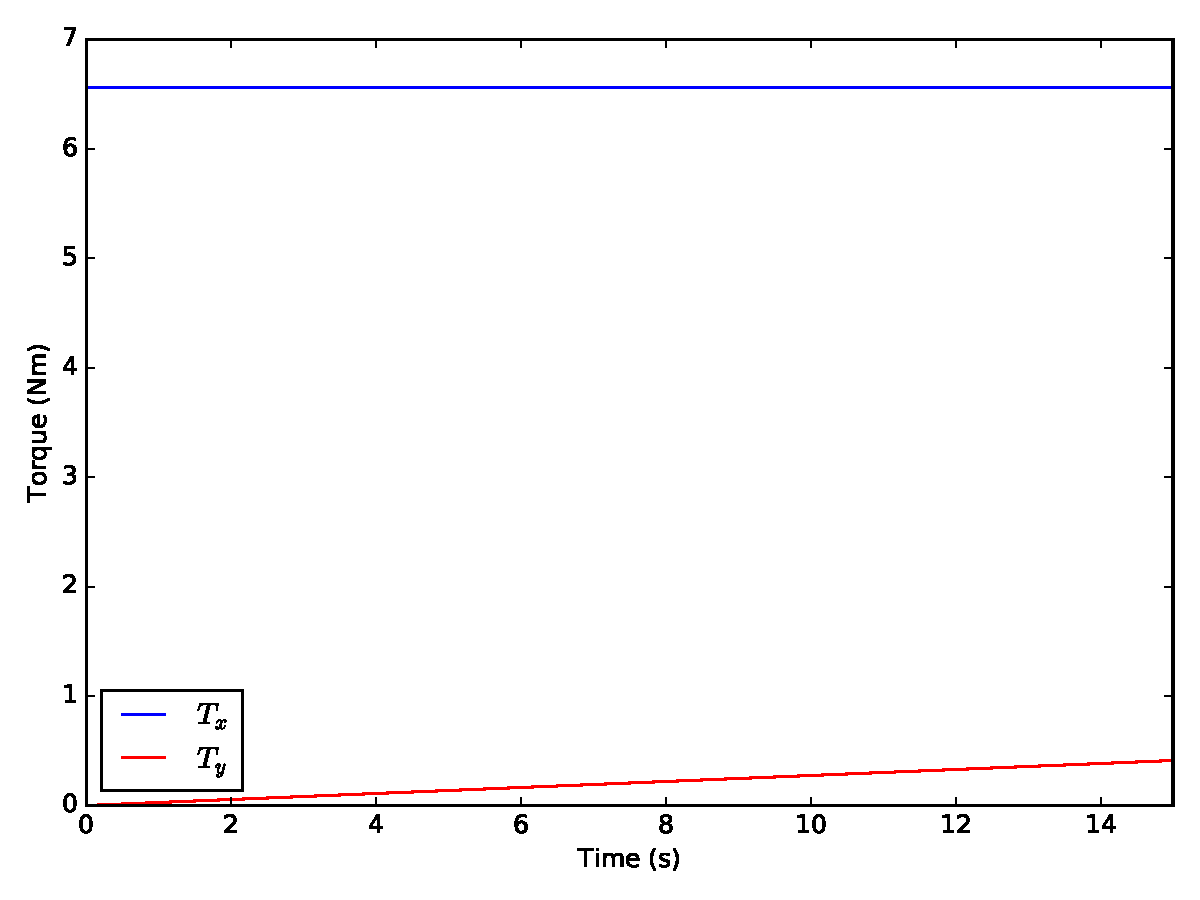
\includegraphics[height=0.45\textheight]{p3_a.pdf}
\end{center}
% \caption{HST Axes Definition for $V_1, V_2, V_3$, CG is located at axis origin}
% \label{fig:on}
\end{figure}

\part{2. Two axis torques}
Find the required variable torque (x) to constantly accelerate the angular precession by 0.1 deg/s$^2$ on the x axis while applying no torque to the y axis.

Plugging in the given values of $I_{wheel} = 1$ kg m$^2$, $\omega = 1500$ rpm, $I_{xx} = 36046$ kg m$^2$ $I_{yy} = 86868$ kg m$^2$, $\dot{\Omega}_x = 0.01$ deg s$^{-2}$, $\Omega_y = 0.1$ deg s$^{-1}$ gives
\begin{align*}
H_{spin} &= 1 \cdot 1500 \cdot 0.1047 = 157.05 \\
T_x &= 36046 \cdot 0.0001745 + 157.05 \cdot \Omega_y \\
T_y &= 86868 \cdot \dot{\Omega}_y + 157.05 \cdot \Omega_x \\
\dot{\Omega}_y &= -\dfrac{157.05 \cdot \Omega_x}{86868} \\
\end{align*}

\begin{figure}[tbh!]
\begin{center}
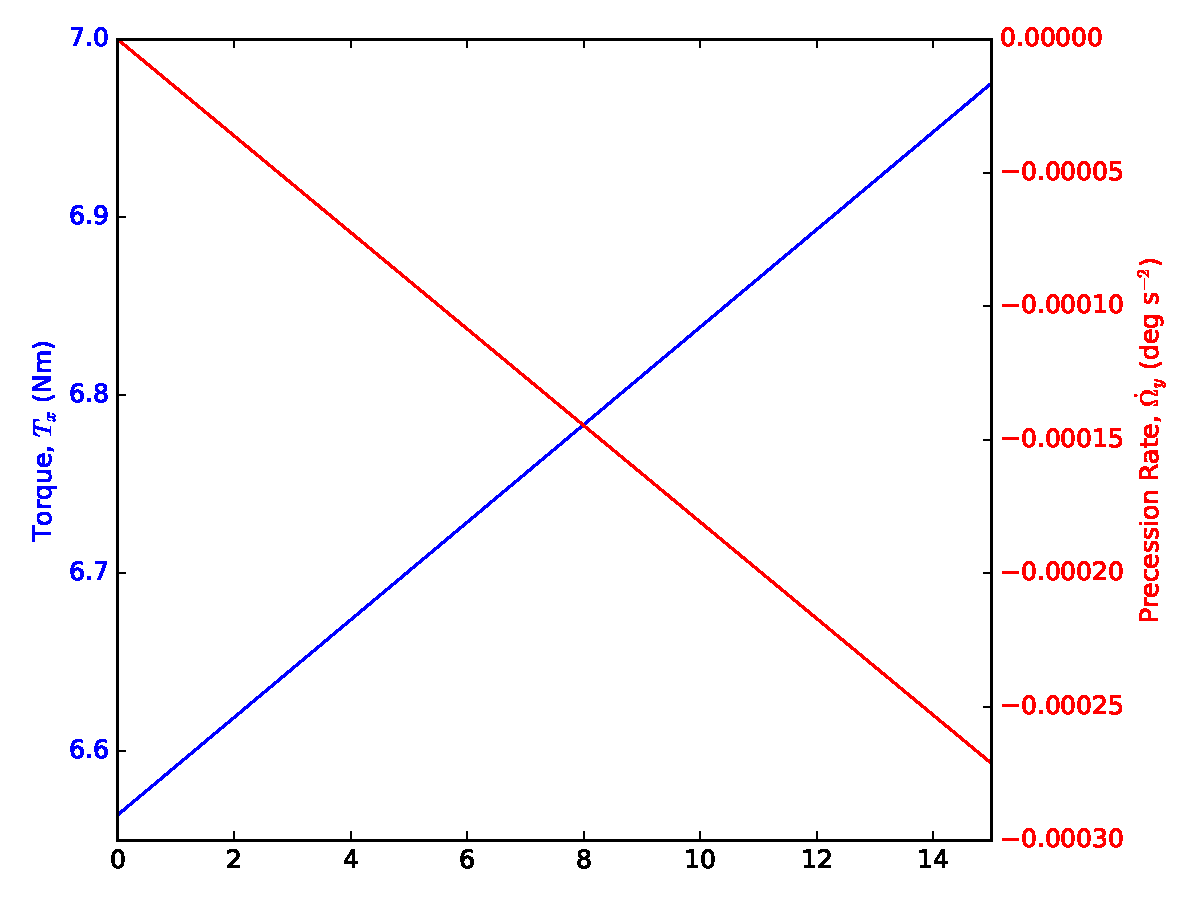
\includegraphics[height=0.45\textheight]{p3_b.pdf}
\end{center}
% \caption{HST Axes Definition for $V_1, V_2, V_3$, CG is located at axis origin}
% \label{fig:on}
\end{figure}

\clearpage
\appendix
\section{Python Code}
\lstinputlisting{hw9.py}


\end{document}
